\section{State of the art}
\label{state}

To get some perspective of the current state of the art with respect to applications related to alcohol intake, three different approaches were taken.

\subsection{Search methods}

\subsubsection{Handsearch}

Some exploration on Google has been done on the field of wearables, such as BACtrack Skyn \cite{bactrackskyn} and Copilot \cite{copiloto}. A later section will deepen on these two wearables.

\subsubsection{Commercial applications}

Firstly, a search through the Apple Store \cite{applestore} was done with three different queries: alcohol, driving, and intake. No applications related to alcohol consumption were found with any of the queries, only driving games and applications to consume more water or measure the intake of calories.
Secondly, a search through the Google Play Store \cite{googleplay} was done with the query alcohol, which threw very interesting results. These results will be reviewed deeper in a later section.

\subsubsection{Scientific publications}

When searching, the terms taken into account were smartphone or similar devices, alcohol or drunkenness and monitor/monitoring and similar. The fields of research were medicine, engineering, psychology and computation. The query used is the one Figure \ref{scopusquery} shows, which threw 231 results on 8th March 2021.

\begin{figure}[h!]
  TITLE-ABS-KEY ( ( smartphone  OR  wearable  OR  smartwatch )  AND  ( alcohol  OR  drunkenness )  AND  ( monitor*  OR  sens*  OR  detect* ) )  AND  ( LIMIT-TO ( PUBYEAR ,  2021 )  OR  LIMIT-TO ( PUBYEAR ,  2020 )  OR  LIMIT-TO ( PUBYEAR ,  2019 )  OR  LIMIT-TO ( PUBYEAR ,  2018 )  OR  LIMIT-TO ( PUBYEAR ,  2017 ) )  AND  ( LIMIT-TO ( SUBJAREA ,  "MEDI" )  OR  LIMIT-TO ( SUBJAREA ,  "ENGI" )  OR  LIMIT-TO ( SUBJAREA ,  "COMP" )  OR  LIMIT-TO ( SUBJAREA ,  "PSYC" ) )
  \caption{Query used in the search through Scopus \cite{scopus}}
  \label{scopusquery}
\end{figure}

Those 231 results were filtered, firstly by the abstract, depending on how interesting the abstract was. This resulted in 63 results after the first filter. These 63 results were once again filtered depending on the accuracy of the abstract according to the subject of our work. Finally,  22 final results were obtained, which were read and a ‘State of Art Matrix’ was built. This matrix can be found in Appendix \ref{appendix:matrix}. After reading the 22 papers, as of 8th March 2021, some very interesting approaches can be analyzed. This proccess is what Figure \ref{proccess} shows.

\begin{figure}[H]
  \centering
  \begin{tikzpicture}
  % NODES
  \tikzset{set/.style={draw,rectangle,inner sep=0pt,align=center}, node distance=1.5cm, minimum height=1cm,minimum width=10cm}
  \node [text centered, rectangle, fill=red!12, draw, rounded corners] (n1) { \textbf{231} unfiltered results (8th March 2021) };
  \node [text centered, rectangle, draw, fill=yellow!20, rounded corners] (n2) [below= of n1]{ \textbf{63} filtered results by interest of abstract };
  \node [text centered, rectangle, draw, fill=green!20, rounded corners] (n3) [below= of n2] { \textbf{22} final results filtered by accuracy of abstract };

  % ARROWS
  \draw [thick,-stealth] (n1) -- node [right,minimum width=1cm] {Filter by abstract} (n2);
  \draw [thick,-stealth] (n2) -- node [right,minimum width=1cm] {Filter by content} (n3);

  \end{tikzpicture}
  \caption{State of the art filtering steps}
  \label{proccess}
\end{figure}

\subsection{Wearables}

BACtrack Skyn \cite{bactrackskyn} is a wearable, a smart bracelet, only available for research, that tracks Transdermal Alcohol Content (TAC) in real time. It can be used on its own or integrated with Apple Watch \cite{applewatch}. It has a cloud-based web portal used to manage, view and export the data obtained with the device. More information can be requested to the BACtrack team on their webpage.

Copilot \cite{copiloto} is a watch and application tandem that allows the user to monitor and learn their driving patterns so it can detect when the pattern changes because of alcohol intake thanks to the watch’s gyroscope, accelerometer and heartbeat monitor.


\subsection{Applications}

As previously mentioned, none of the results when searching through the Google Play \cite{googleplay} were interesting. On the other hand, it is interesting to deepen on the results of the search through the Google Play \cite{googleplay}. The next paragraphs deepen on these results.

\begin{figure}[H]
  \centering
  \begin{subfigure}{0.3\textwidth}
      \centering
      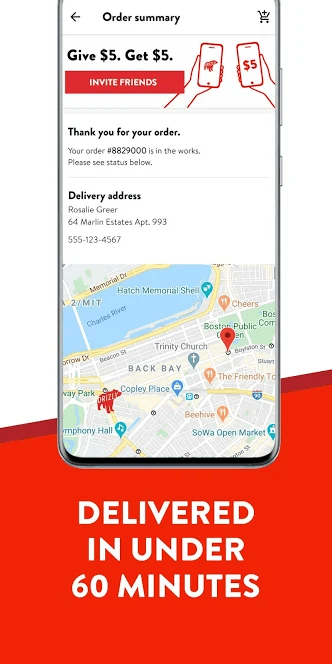
\includegraphics[width=0.8\textwidth]{./img/Drizly.png}
      \caption{Drizly \cite{Drizly} application}
      \label{Drizly}
  \end{subfigure}\hfill
  \begin{subfigure}{0.38\textwidth}
      \centering
      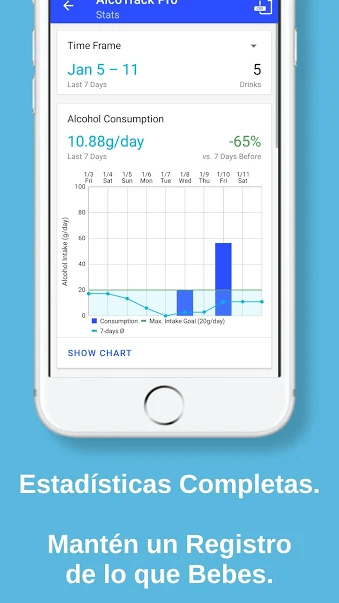
\includegraphics[width=0.8\textwidth]{./img/Alcotrack.png}
      \caption{Alcotrack \cite{alcotrack} application}
      \label{Alcotrack}
  \end{subfigure}
  \begin{subfigure}{0.3\textwidth}
      \centering
      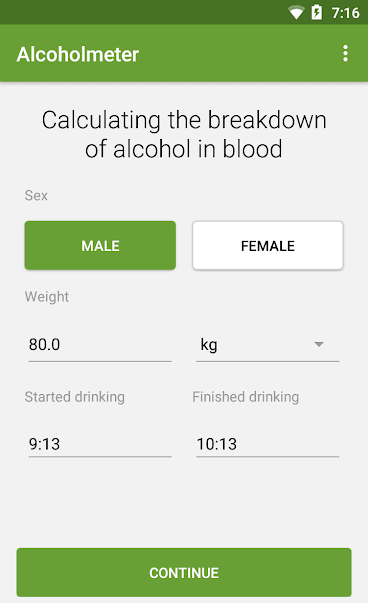
\includegraphics[width=0.8\textwidth]{./img/Alcoholcheck.png}
      \caption{Alcoholcheck \cite{alcoholcheck} application}
      \label{Alcoholcheck}
  \end{subfigure}

%//

  \begin{subfigure}{0.3\textwidth}
      \centering
      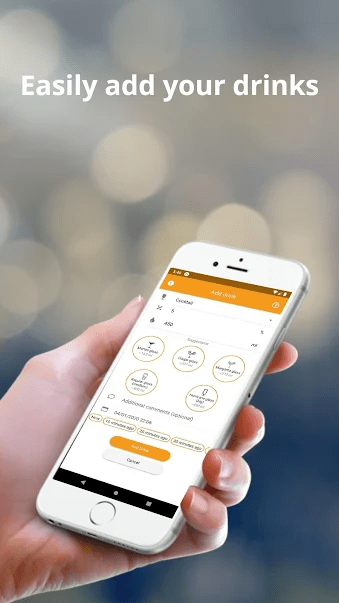
\includegraphics[width=0.65\textwidth]{./img/alcofy.png}
      \caption{Alcofy \cite{Alcofy} application}
      \label{Alcofy}
  \end{subfigure}\hfill
  \begin{subfigure}{0.38\textwidth}
      \centering
      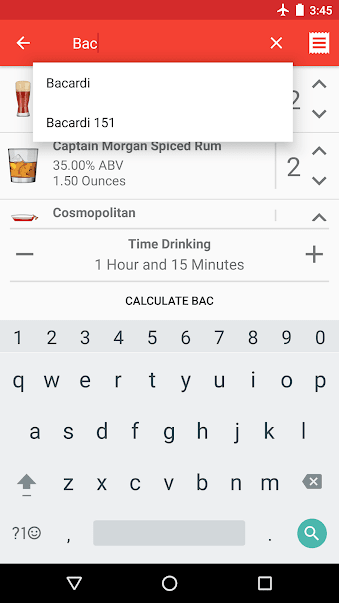
\includegraphics[width=0.5\textwidth]{./img/alcoholcalculator.png}
      \caption{Blood Alcohol Calculator \cite{alcoholcalculator} application}
      \label{alcoholcalculator}
  \end{subfigure}
  \begin{subfigure}{0.3\textwidth}
      \centering
      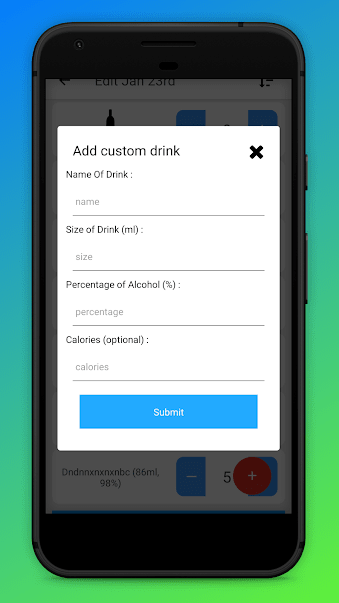
\includegraphics[width=0.65\textwidth]{./img/saut.png}
      \caption{Simple Alcohol Unit Tracker \cite{saut} application}
      \label{saut}
  \end{subfigure}

%//

  \begin{subfigure}{0.3\textwidth}
      \centering
      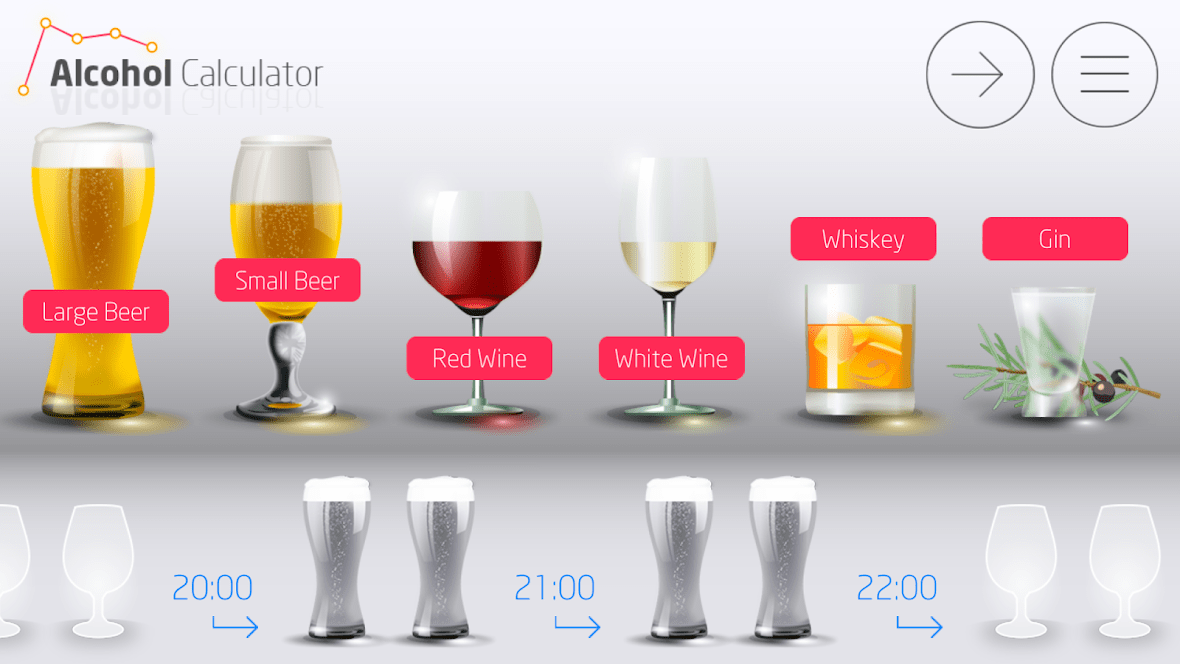
\includegraphics[width=1.1\textwidth]{./img/calculator.png}
      \caption{Blood Alcohol Calculator \cite{calculator} application}
      \label{calculator}
  \end{subfigure}\hfill
  \begin{subfigure}{0.38\textwidth}
      \centering
      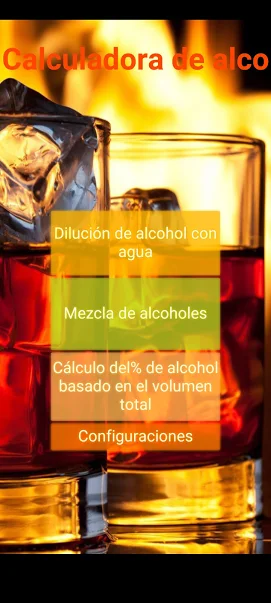
\includegraphics[width=0.4\textwidth]{./img/alcocal.png}
      \caption{Alco Calculator \cite{alcocal} application}
      \label{AlcoCalculator}
  \end{subfigure}
  \begin{subfigure}{0.3\textwidth}
      \centering
      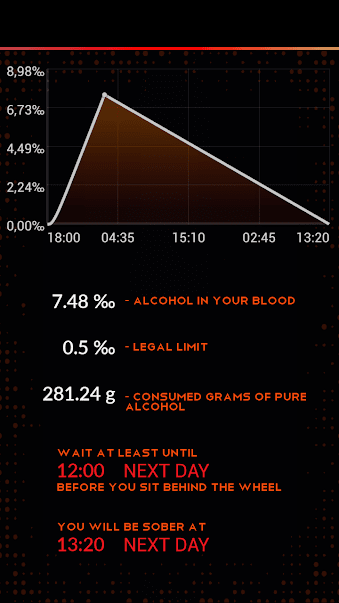
\includegraphics[width=0.65\textwidth]{./img/forfun.png}
      \caption{Alcohol test (for fun) \cite{forfun} application}
      \label{forfun}
  \end{subfigure}
  \caption{Screenshots of the different applications found in the Google Play \cite{googleplay}}
  \label{Screenshots}
\end{figure}

\newpage

  Drizly \cite{Drizly} is an application where the user can select different alcoholic beverages and get them delivered home. Alcotrack \cite{alcotrack} tracks alcohol consumption through self-report of alcoholic drinks. Alcoholcheck \cite{alcoholcheck} calculates blood alcohol content and an estimate of how long it will take you to reach zero level of alcohol in blood again after inserting gender, age, weight and consumed beverages.
  Alcofy \cite{Alcofy} is an application to add drinks in real time to see how drunk the user is and will be the next hours until they become sober. A limit can be set and the application will send a warning if the user is about to cross that limit. The estimated blood alcohol concentration is calculated based on a formula that has been studied and praised in scientific papers. Blood Alcohol Calculator \cite{alcoholcalculator} is an application to add weight, gender, drinks selected from a list of hundreds of built-in drinks or created/customized by the user and how long the user has been drinking to calculate the blood alcohol content of you and your friends. This shows the estimation of blood alcohol concentration and some possible side effects related to that blood alcohol range, as well as a detailed graph letting you know what your blood alcohol content will be over time. Simple Alcohol Unit Tracker \cite{saut} calculates the approximate blood alcohol concentration level based on the information about the user and their consumed alcoholic drinks. It has several options: calculation of blood alcohol concentration, reflex test, addition of new alcohol types and the setting of alcohol limits.
  Blood Alcohol Calculator \cite{calculator} calculates blood alcohol content and an estimate of how long it will take you to reach zero level of alcohol in blood again after inserting gender and consumed beverages. Alco Calculator \cite{alcocal} calculates the concentration of alcohol in a disolution (beverage or not). Alcohol test (for fun) \cite{forfun} is an application to add drinks and understand their alcohol consumption/drinking habits. A screenshot of each of these applications can be found in Figure \ref{Screenshots}.


\subsection{Scientific articles}

With respect to scientific articles found in Scopus \cite{scopus} and filtered as previously mentioned, different aspects have been taken into account:

\subsubsection{Countries from the affiliations}

Most of the affiliations are exclusively from USA \cite{Li2021,Mitchell2020297,Businelle2020,Suffoletto2020505,Killian201935,Willoughby2019496,Mariakakis2018,Suffoletto2018116,Leonard2017,Kinnamon2017}, but others were a colaboration of one or more countries out of the USA and a country from USA \cite{Sempionatto2019161,Bertholet2017285,Park201774}. Only three articles have affiliations exclusively from UK and those are \cite{Leightley2020,Garnett2019296,Leightley2018}. Australia participated in \cite{Poulton201835} and with Switzerland in \cite{Phan2020211}. Japan was the country of the affiliations of \cite{Wakana2019}, India was the country of affiliation of \cite{Chatterjee2018} and Denmark of \cite{Mellentin2017}. Table \ref{countries} summarizes the relation between countries and affiliations.

\begin{table}[h!]
  \centering
 \begin{tabular}{|| c | c ||}
 \hline
 \textbf{Country} & \textbf{Affiliations (out of 22)} \\ [0.5ex]
 \hline\hline
 USA & 13\\
 \hline
 UK & 4\\
 \hline
 Autralia & 3\\
 \hline
 Switzerland &  2\\
 \hline
 Brazil & 1\\
 \hline
 Canada & 1\\
 \hline
 Denmark & 1\\
 \hline
 Japan & 1\\
 \hline
 India & 1\\
 \hline
 South Korea & 1\\
 \hline
 Spain & 1\\
 \hline
 Thailand & 1\\ [0.5ex]
 \hline
\end{tabular}
\caption{Affiliations' countries of the different studies reviewed}
\label{countries}
\end{table}

\subsubsection{Sample size}

Most of the studies had a sample of less than 100 people summing all of the mentioned phases of the study, specifically 13 out of the 22 studies previously mentioned \cite{Li2021,Intarasirisawat2020,Mitchell2020297,Suffoletto2020505,Leightley2020,Killian201935,Sempionatto2019161,Leightley2018,Mariakakis2018,Suffoletto2018116,Leonard2017,Mellentin2017,Park201774}. Four of them \cite{Wakana2019,Garnett2019296,Chatterjee2018,Kinnamon2017} did not mention anything about the sample used in the study and the remaining five had samples between 120 and 671 subjects \cite{Phan2020211,Businelle2020,Willoughby2019496,Poulton201835,Bertholet2017285}. More information can be found in the Appendix \ref{appendix:matrix}.

\subsubsection{Diversity}

According to diversity, three different aspects were taken into account: age diversity, gender diversity and ethnic diversity.

Regarding age, eight of them \cite{Businelle2020,Wakana2019,Sempionatto2019161,Willoughby2019496,Garnett2019296,Chatterjee2018,Mellentin2017,Park201774} did not mention anything about the ages of the samples. Most of the rest have a wide age range, but four of them \cite{Phan2020211,Killian201935,Suffoletto2018116,Leonard2017} were specifically for young people therefore the age range was more limited.
Regarding gender, eight of them \cite{Businelle2020,Leightley2020,Wakana2019,Sempionatto2019161,Garnett2019296,Chatterjee2018,Mellentin2017,Park201774} did not mention anything about the gender and one mentioned diversity but did not mention ratios nor percentages. One had a 100\% of males with no specific reason \cite{Intarasirisawat2020} and another one had 100\% of females because the study wanted to study the impact of problematic alcohol drinking in female college students \cite{Leonard2017}. The rest of the studies were approximately half male and half female (some had up to 70\% one gender), except one \cite{Leightley2018}, that has almost 90\% male and only almost 10\% female.
Regarding ethnic, more than half of the studies, 15 out of 22 \cite{Li2021,Intarasirisawat2020,Phan2020211,Mitchell2020297,Leightley2020,Wakana2019,Sempionatto2019161,Willoughby2019496,Garnett2019296,Chatterjee2018,Leightley2018,Poulton201835}, did not mention anythihng about ethnic, four of them \cite{Businelle2020,Suffoletto2020505,Mariakakis2018,Bertholet2017285} mentioned diversity but did not specified proportions nor percentages and the rest were diverse. More information can be found in the Appendix \ref{appendix:matrix}.

\subsubsection{Applications}

Less than a fourth of the studies, 5 out of 22 \cite{Suffoletto2020505,Sempionatto2019161,Chatterjee2018,Kinnamon2017,Park201774}, did not use any smartphone application. One of the remaining studies \cite{Intarasirisawat2020} used pre-existing applications: Tetris, Fruit Ninja, and Unblock Puzzle, all three of them with some modifications to track important information; another 5 studies \cite{Phan2020211,Businelle2020,Wakana2019,Killian201935,Mellentin2017} used an application but did not mention the name and the rest used the following applications: Alcogait \cite{Li2021}, Ria Treatment Platform app \cite{Mitchell2020297}, Drinks:Ration \cite{Leightley2020}, DrunkSelfie \cite{Willoughby2019496}, Drink Less \cite{Garnett2019296}, InDEx (Information about Drinking for Ex-serving personnel) \cite{Leightley2018}, CNLab-A \cite{Poulton201835}, DUI (Drunk user interfaces) \cite{Mariakakis2018}, DrinkTRAC \cite{Suffoletto2018116}, Empatica \cite{Leonard2017} and Alcooquizz \cite{Bertholet2017285}.

\subsubsection{Device(s)}

Regarding devices, some of the studies used only smartphones \cite{Intarasirisawat2020,Phan2020211,Mitchell2020297,Suffoletto2020505,Wakana2019,Willoughby2019496,Garnett2019296,Chatterjee2018,Leightley2018,Poulton201835,Mariakakis2018,Suffoletto2018116,Bertholet2017285,Mellentin2017} and some others used smartphones and some kind of wearable \cite{Li2021,Businelle2020,Leightley2020,Killian201935,Leonard2017}. Only \cite{Park201774}, \cite{Sempionatto2019161} and \cite{Kinnamon2017} used only wearables (smart shoes, smart eyeglasses and electronic bracelet, respectively). Table \ref{devices} summarizes the devices and sensors used in the reviewed studies. More information can be found in the matrix attached in the Appendix \ref{appendix:matrix}.

\begin{longtable}[h!]{||p{.2\textwidth} | p{.25\textwidth} | p{.25\textwidth}| p{.25\textwidth}||}
\caption{Smartphone specifications  and measurements from smartphones used in the reviewed studies}
\label{devices}
\endfirsthead
\hline
\textbf{Study} & \textbf{Device(s)} & \textbf{Sensors} & \textbf{Measurements} \\
\hline
\hline
\endhead
\hline
\textbf{Study} & \textbf{Device(s)} & \textbf{Sensors} & \textbf{Measurements} \\
\hline
Li et al. (2021) \cite{Li2021} & Smartphone (Google Pixel XL) + wearable (LG Watch Sport) & \multirow{2}{=}{Accelerometer and gyroscope} & Gait changes \\ \cline{1-2} \cline{4-4}
Intarasirisawat et al. (2020) \cite{Intarasirisawat2020} & Smartphone (Samsung S6) &  & Device acceleration, rotational motion and touch-based features \\ \hline
Phan et al. (2020) \cite{Phan2020211} & Smartphone (Model not specified, Android OS) & Accelerometer, Bluetooth, WiFi, GPS, apps logs, camera & Location accuracy, speed, and GPS coordinates, network percentage; and mobility. human mobility, social context and person-person proximity \\ \hline
Mitchell et al. (2020) \cite{Mitchell2020297} & Smartphone (Model not specified and OS not specified) & Breathalyzer (External) & Alcohol in breath \\ \hline
Businelle et al. (2020) \cite{Businelle2020} & Smartphone (Samsung Galaxy J3 smartphone (or equivalent)) + wearable (SCRAM bracelet) & Geolocation & Longitude + latitude (geolocation), BAC  \\ \hline
Suffoletto et al. (2020) \cite{Suffoletto2020505} & Smartphone (Model not specified and OS not specified) & Accelerometer & Mean of acceleration signal, Variance of acceleration signal, Correlation of pairwise acceleration signals, Covariance of acceleration signal, Maximum difference of acceleration signal, Maximum difference of pairwise acceleration signals, Mean trend of acceleration signal of 0.1 second windows within the window, Windowed mean trend of acceleration signal of 0.1 second windows within the window, Variance trend of acceleration signal, Windowed variance trend of acceleration signal \\ \hline
Leightley et al. (2020) \cite{Leightley2020} & Smartphone (Model not specified, Android and iOS OS) + wearable (not specified) & GPS, push notifications & Location, heart rate, distance travelled, activities, height, and weight \\ \hline
Wakana \& Yamada (2019) \cite{Wakana2019} & Smartphone (Model not specified and OS not specified) & Breathalyzer (External) & Breath Alcohol Concentration (BrAC) \\ \hline
Killian et al. (2019) \cite{Killian201935} & Smartphone (Model not specified, Android and iOS OS) wearable (SCRAM bracelet) & Accelerometer & Acceleration/movement and TAC (transdermal alcohol content) \\ \hline
Sempionatto et al. (2019) \cite{Sempionatto2019161} & Wearable (smart glasses) & Alcohol biosensor and amperometric sensor & Alcohol and Glucose in tears \\ \hline
Willoughby et al. (2019) \cite{Willoughby2019496} & Smartphone (Model not specified, Android OS) & Camera & Face Detection, Locating Facial Landmarks, Aligning Faces using Landmarks, Landmark positions, Landmark vectors, Landmark lines, Detecting facial lines and wrinkles using Canny Edge detection and the Hough transform, Forehead redness, Smiles, Lips and Eyes \\ \hline
Garnett et al. (2019) \cite{Garnett2019296} & Smartphone (Model not specified, iOS OS) & None & ABV (alcohol by volume), size, quantity and price. Mood, productivity, clarity and sleep quality. Calorie intake, spend on alcohol, and how mood, productivity, clarity and sleep quality are affected by heavy drinking. \\ \hline
Chatterjee, Isha and Sharma (2018) \cite{Chatterjee2018} & Smartphone (Model not specified and OS not specified) & Camera & Video of the person \\ \hline
Leightley et al. (2018) \cite{Leightley2018} & \multirow{2}{=}{Smartphone (Model not specified, Android and iOS OS)} & \multirow{2}{=}{None} & Amount of alcohol consumed, how and when \\ \cline{1-1} \cline{4-4}
Poulton et al. (2018) \cite{Poulton201835} & &  & Quantity, frequency, type of alcohol, start and finish times \\ \hline
Mariakakis et al. (2018) \cite{Mariakakis2018} & Smartphone (Third-generation Moto G smartphone) & Touchscreen, accelerometer, and gyroscope, flash and camera & How correctly they write and if they correct or not the mistakes, also how the subject maintain the balance, heart rate \\ \hline
Suffoletto et al. (2018) \cite{Suffoletto2018116} & Smartphone (Model not specified, iOS OS) & Accelerometer, gyroscope and magnetometer & Real, dynamic and static acceleration, angular velocity, attitude of the device \\ \hline
Leonard et al. (2017) \cite{Leonard2017} & Smartphone (Model not specified, Android OS) wearable (Empatica E4 wrist band) & Electrodermal activity (EDA), accelerometer and temperature sensor & Real-time EDA, movement, temperature, heart rate \\ \hline
Bertholet et al. (2017) \cite{Bertholet2017285} & Smartphone (Model not specified, Android and iOS OS) & None & Quantity and frequency of alcohol consumption \\ \hline
Kinnamon et al. (2017) \cite{Kinnamon2017} & Wearable (Electronic Bracelet for Monitoring of Alcohol Lifestyle) & Immunoassay based EtG biosensor & Ethyl glucuronide (EtG) in sweat \\ \hline
Mellentin et al. (2017) \cite{Mellentin2017} & Smartphone(Model not specified, Android OS) & App logs & Real-time measures of cue-induced cravings. \\ \hline
Park et al. (2017) \cite{Park201774} & Wearable (smart shoes) & Array of pressure sensors & Pressure of the feet when walking \\ \hline
\end{longtable}


As shown in Table \ref{devices}, more than a fifth are multiplatform, available for both Android and iOS, almost a fifth works for Android and almost a fifth does not specify the operative system. Some of them have specific models, like Samsung S6, Samsung Galaxy J3 (or equivalent), Third-generation Moto G and Google Pixel XL. Table \ref{smartphonespecifications} sums up the different devices used along the studies. Not a lot of wearables are used. Some of them are SCRAM bracelet, Empatica E4 wrist band and LG Watch Sport. Table \ref{wearables} summarizes the different wearables used in the reviewed studies.

\begin{table}[h!]
  \centering
 \begin{tabular}{||c | c ||}
 \hline
 \textbf{Smartphone specifications} & \textbf{Studies (out of 22)} \\ [0.5ex]
 \hline \hline
  Model not specified, Android and iOS &  5\\
  \hline
 Model and OS not specified & 4\\
 \hline
 Model not specified, Android OS & 4\\
 \hline
 Model not specified, iOS OS & 2\\
 \hline
 Samsung S6 & 1\\
 \hline
 Samsung Galaxy J3 (or equivalent) & 1\\
 \hline
 Third-generation Moto G & 1\\
 \hline
 Google Pixel XL & 1\\[0.5ex]
 \hline
\end{tabular}
\caption{Smartphone specifications from smartphones used in the reviewed studies}
\label{smartphonespecifications}
\end{table}

\begin{table}[h!]
  \centering
 \begin{tabular}{||c | c ||}
 \hline
 \textbf{Wearables} & \textbf{Studies (out of 22)} \\ [0.5ex]
 \hline\hline
 SCRAM bracelet & 2\\
 \hline
 LG Watch Sport & 1\\
 \hline
 Not specified & 1\\
 \hline
 Empatica E4 wrist band &  1\\
 \hline
 Electronic Bracelet for Monitoring of Alcohol Lifestyle & 1\\[0.5ex]
 \hline
\end{tabular}
\caption{Wearables used in the reviewed studies}
\label{wearables}
\end{table}

\subsubsection{Sensors}

The most used sensors are accelerometer and gyroscope, but also geolocation, camera and temperature sensors. Some of the studies do not mention the use of any kind of sensors \cite{Garnett2019296,Leightley2018,Poulton201835,Bertholet2017285}. Table \ref{sensors} summarizes the use of sensors. More  information can be found in table \ref{devices} and in the Appendix \ref{appendix:matrix}.

\begin{table}[h!]
  \centering
 \begin{tabular}{||c | c ||}
 \hline
 \textbf{Sensors} & \textbf{Studies (out of 22)} \\ [0.5ex]
 \hline\hline
 Accelerometer & 8\\
 \hline
 Gyroscope & 4\\
 \hline
 Camera & 3\\
 \hline
 Application logs &  2\\
 \hline
 Geolocation &  2\\
 \hline
 Breathalyzer & 2\\
 \hline
 Bluetooh & 1\\
 \hline
 WiFi &  1\\
 \hline
 Flash & 1\\
 \hline
 Push notifications & 1\\
 \hline
 Alcohol biosensor & 1\\
 \hline
 Amperometric sensor & 1\\
 \hline
 Touchscreen &  1\\
 \hline
 Magnetometer & 1\\
 \hline
 Electrodermal activity (EDA) & 1\\
 \hline
 Temperature & 1\\
 \hline
 Immunoassay based EtG biosensor &  1\\
 \hline
 Pressure &  1\\
 \hline
 None & 4\\[0.5ex]
 \hline
\end{tabular}
\caption{Sensors \cite{Businelle2020} used in the reviewed studies}
\label{sensors}
\end{table}


\subsubsection{Mobile self-report}

Almost half of the studies (10 out of 22) use mobile self-report as an information collector. Of those 10 studies, in 8 of them \cite{Phan2020211,Businelle2020,Leightley2020,Garnett2019296,Leightley2018,Poulton201835,Suffoletto2018116,Bertholet2017285} the user added information about alcohol consumption: type of alcohol, amount of beverage, time elapsed when drinking...; one \cite{Leonard2017} asked for information about feelings when a notification popped up and the last one \cite{Mellentin2017} was about cravings when staring at alcoholic beverages. More information can be found in the Appendix \ref{appendix:matrix}.

\subsubsection{Measurements}

Most of the measurements taken are physical ones, related to location and motion like acceleration and movement, but also measurements related to drinking like quantity, frequency, type of alcohol and start and finish times when drinking. Also alcohol in blood, breath and transdermal are meassured. Some studies use videos \cite{Chatterjee2018} or selfies \cite{Willoughby2019496} of the user. More information can be found in table \ref{devices} and in the Appendix \ref{appendix:matrix}.

\subsubsection{Methods}

Table \ref{methods} summarizes the methods to proccess the previously mentioned data gathered from the sensors and the output obtained with this proccesses.

\begin{longtable}{||p{.2\textwidth} | p{.25\textwidth} | p{.25\textwidth} | p{.25\textwidth}||}
\caption{Methods to proccess measurements and outputs from them in the reviewed studies}
\label{methods}
\endfirsthead
\hline
\textbf{Study} & \textbf{Methods} & \textbf{Output} & \textbf{Drawbacks} \\
\hline
\hline
%
\endhead
\hline
\hline
\textbf{Study} & \textbf{Methods} & \textbf{Output} & \textbf{Drawbacks} \\ \hline
Li et al. (2021) \cite{Li2021} & Machine Learning & Warning while drinking/on the way to the car & Possible bias in layer normalization and methods towards certain subjects \\ \hline
Intarasirisawat et al. (2020) \cite{Intarasirisawat2020} & Machine Learning & Visualization & No gender diversity. Exclusion of people with different conditions. Small sample of study/control. \\ \hline
(Phan, Labhart, Muralidhar \& Gatica-Perez, 2020) \cite{Phan2020211} & Machine learning & Classifiication of the consumption: heavy or non-heavy drinking & No assurance data is correctly inserted, bias in self-report \\ \hline
Mitchell et al. (2020) \cite{Mitchell2020297} & Statistics & Models for the relationship between BAC and time & No control group. Patients were highly motivated. Approximately 46\% of data for the BAC readings were missing.\\ \hline
Businelle et al. (2020) \cite{Businelle2020} & Others & Text messages to in-the-moment distraction, reframing, immediate help-seeking, planning, and other tools to reduce craving. & The intervention app may not be applicable to those with low literacy and cognitive impairment. EMA or SCRAM monitoring may have independent effects on drinking. Self-monitoring can lead to changes in drinking, even without an “intended” intervention. \\ \hline
Suffoletto et al. (2020) \cite{Suffoletto2020505} & Machine Learning & Models, regressions and predictions of excessive alcohol consumption & Small sample size, the use of a cohort that largely drinks below risky levels, and controlled setting of data measurement. It did not examine whether gait-related features discriminate lower levels of drinking. It placed the smartphone on the lower back, which may not represent where individuals keep their phones in natural environments. Did not find that population-based models were accurate in predicting intoxication. \\ \hline
Leightley et al. (2020) \cite{Leightley2020} & Statistics & Push notifications/ SMSs to warn/inform the subject & \multirow{2}{*}{-} \\ \cline{1-3}
Wakana \& Yamada (2019) \cite{Wakana2019} & Others & Estimated BrAC and detection of saturated water vapor and the metabolites &  \\ \hline
Killian et al. (2019) \cite{Killian201935} & Machine Learning & Clasification of sobriety every 10 seconds. & Low control of the phone placement, low accuracy of accelerometer, classifiers had a higher accuracy for sober data than intoxicated data and that the variance of the best classifier was high for intoxicated subjects.\\ \hline
Sempionatto et al. (2019) \cite{Sempionatto2019161} & Others & Estimation of glucose and alcohol in blood & Small sample size. small sample volumes of the extracted tears, ease of sample evaporation during collection (particularly in sampling ethanol), potential composition variations between individuals and dependence on the sampling method. \\ \hline
Willoughby et al. (2019) \cite{Willoughby2019496} & Machine Learning & Classification of images: drunk or sober & Limited Dataset, Coarse Classification, Smartphone Internet Access Requirement and Comprehensive evaluation of DrunkSelfie app by users \\ \hline
Garnett et al. (2019) \cite{Garnett2019296} & Basic statistics & Feedback and graphics about goals. & \multirow{2}{*}{-} \\ \cline{1-3}
Chatterjee, Isha and Sharma (2018) \cite{Chatterjee2018} & Computer vision techniques of facial landmark detection and motion detection & Alert sound and location notification if the subject is drunk or drowsy &  \\ \hline
Leightley et al. (2018) \cite{Leightley2018} & Basic statistics & SMS with information and warnings, statistics of usage of the application and visualization of data from the reports & No assurance data is correctly inserted, not a long-term analysis, sample is very small, possible selection bias of the participants \\ \hline
Poulton et al. (2018) \cite{Poulton201835} & Statistics & Average daily and weekly consumption, hourly rate of consumption each day, days of consumption, total drinks and days in which 4 or 6 or 8 or (and so forth) more drinks were drunk & Limited alcohol options, no assurance data is correctly added \\ \hline
Mariakakis et al. (2018) \cite{Mariakakis2018} & Machine learning & Estimation of BAL (Blood alcohol level) & It doesn't meassure BAL directly \\ \hline
Suffoletto et al. (2018) \cite{Suffoletto2018116} & Machine Learning & Accurate prediction of blood alcohol concentration during drinking episodes & Sample is very small. Missing gait task data. Participants were paid to complete tasks, which likely artificially inflated completion rates. App was made only for iOS devices. Possible wrong insertion of alcohol drinks. \\ \hline
Leonard et al. (2017) \cite{Leonard2017} & Psycological & Analysis of the emotion + context, sum of use of screen with the app, amount of reports & Sample is very small. The form of the band was not accurate and the participants often forgot to charge it. The connection was not great and some alerts were inopportune \\ \hline
Bertholet et al. (2017) \cite{Bertholet2017285} & Statistics & Statistics about alcohol consumption habits & The uncontrolled design does not allow us to infer causation, further study is needed to evaluate the application's efficacy. Assessment of alcohol consumption relied on self-report, therefore social desirability bias or recall bias are possible. Assessment of app use also relied on self-report. \\ \hline
\pagebreak
Kinnamon et al. (2017) \cite{Kinnamon2017} & Electrochemical & Visualization of graphs with information about voltage, intensity and EtG concentration & \multirow{3}{*}{-} \\ \cline{1-3}
Mellentin et al. (2017) \cite{Mellentin2017} & Basic statistics & Measures and graphs to keep track of their training activities and potential advances in controlling cue reactivity &  \\ \cline{1-3}
Park et al. (2017) \cite{Park201774} & Machine Learning & A pressure distribution map and classification of the gait &  \\ \hline
\end{longtable}

Most of the studies use machile learning techniques like Logistic Regression (LR), Linear Support Vector Machine (LSVM), Random Forest (RF), Bi-directional Long Short Term Memory (Bi-LSTM) and Convolutional Neural Network (CNN), in addition to Cross-Validation (CV).
Statistics like average, median, summations, t-tests and chi-square tests are also used by some studies.
\cite{Kinnamon2017} uses square wave voltammetry (SWV), an electrochemical methods, \cite{Chatterjee2018} uses computer vision techniques of facial landmark detection and motion detection.
Others use techniques such as tears estimulation and alcohol and glucose detection in tears like \cite{Sempionatto2019161}, questionnaires for developing + 'real time' drinking algorithm for testing like \cite{Businelle2020} or a calculation algorithm based on a differential evolutional method like \cite{Wakana2019}. The summary of the usage of these methods can be seen in table \ref{studymethods}.

\begin{table}[h!]
  \centering
 \begin{tabular}{||c | c ||}
 \hline
 Method & Studies (out of 22) \\ [0.5ex]
 \hline\hline
 Machine Learning & 9\\
 \hline
 Statistics & 7\\
 \hline
 Computer vision techniques & 1\\
 \hline
 Psycological &  1\\
 \hline
 Electrochemical &  1\\
 \hline
 Others & 3\\[0.5ex]
 \hline
\end{tabular}
\caption{Methods used in the studies}
\label{studymethods}
\end{table}

\subsubsection{Output}

There is a wide range of outputs, from visualization to classification, but also notifications, models for the relationship between drinking and time estimations of alcohol in blood. More information can be found in Table \ref{methods} and in the Appendix \ref{appendix:matrix}.

\subsubsection{Drawbacks}

The most common drawbacks are the small sample size and the lack of control of some variables, like low control of the phone placement, low accuracy of accelerometer or no assurance data is correctly inserted. More information can be found in Table \ref{methods} and in the Appendix \ref{appendix:matrix}.

\subsubsection{Conflicts of interest}

None of the above mentioned articles had any conflicts of interest but these four:

\begin{itemize}
  \item John Mendelson is the owner of Ria Health. The remaining authors have nothing to disclose \cite{Mitchell2020297}.
  \item MB is an inventor of the Insight mHealth Platform and receives royalties related to use of this platform \cite{Businelle2020}.
  \item NTF sits on the Independent Group Advising on the Release of Data at NHS Digital. NTF is also a trustee of a military-related charity. AS is a full-time member of the Armed Forces seconded to King’s College London. DM and CW are employed by Combat Stress, a national charity in the United Kingdom that provides clinical mental health services to veterans \cite{Leightley2020}.
  \item J.B. has received unrestricted research funding from Pfizer related to smoking cessation. R.W. has received research funding and undertaken consultancy for companies that manufacture smoking cessation medications. R.W. and S.M. are advisers to the National Centre for Smoking Cessation and Training. S.M. is Director of the UCL Centre for Behaviour Change \cite{Garnett2019296}.
\end{itemize}

\newpage
